\documentclass[a4paper,11pt]{article}
\usepackage[a4paper,margin=2.4cm]{geometry}
\setlength{\emergencystretch}{2em}
\usepackage{amsmath,amssymb,amsthm}
\usepackage{fontspec}
\usepackage{unicode-math}
\usepackage{graphicx}
\usepackage{booktabs}
\usepackage{hyperref}
\usepackage{xcolor}
\definecolor{neonmagenta}{HTML}{FF10F0}
\usepackage{enumitem}
\usepackage{seqsplit}
\usepackage{fvextra}
% Allow long filenames to break across lines
\newcommand{\filename}[1]{\texttt{\seqsplit{#1}}}
% fvextra Verbatim for Lean listings (Unicode-safe, keeps characters in order)
\newcounter{leanlisting}
\newenvironment{leanlisting}[2]{%
  \refstepcounter{leanlisting}\label{#2}%
  \begin{center}\textit{\small Listing \theleanlisting: #1}\end{center}%
  \Verbatim[breaklines=true,breakanywhere=true,fontsize=\footnotesize,frame=single,framesep=4pt,rulecolor=\color{gray!50},fillcolor=\color{gray!5}]%
}{%
  \endVerbatim%
}
% Portable fonts: system font names, no hardcoded paths.
% Fira ONLY (Brandon 2026-10-01): Fira Sans (text), Fira Mono (code),
% Fira Math (math, with FakeBold=0.3). Latin Modern Math is FORBIDDEN
% everywhere, including inside tabular environments.
\setmainfont{Fira Sans}[BoldFont={Fira Sans Bold},ItalicFont={Fira Sans Italic},BoldItalicFont={Fira Sans Bold Italic}]
\setmonofont{Fira Mono}[BoldFont={Fira Mono Bold}]
\setmathfont{Fira Math}[FakeBold=0.3,Scale=1.08]
\usepackage{etoolbox}
\hypersetup{colorlinks=true,linkcolor=blue!60!black,citecolor=blue!60!black,urlcolor=blue!60!black}
\setlength{\parskip}{0.6em}
\setlength{\parindent}{0pt}
\setlength{\emergencystretch}{2em}

\theoremstyle{plain}
\newtheorem{theorem}{Theorem}[section]
\newtheorem{proposition}[theorem]{Proposition}
\newtheorem{lemma}[theorem]{Lemma}
\newtheorem{corollary}[theorem]{Corollary}

\theoremstyle{definition}
\newtheorem{definition}[theorem]{Definition}

\theoremstyle{remark}
\newtheorem{remark}[theorem]{Remark}

\begin{document}

\title{\textbf{\Large Elimination of the GGHV Branch-(c) Normal Form at Degree~Pair $(72,108)$:}\\[0.6em]
\large A Certified Computational Audit\\[0.4em]
\normalsize Descent, Chart Conditions, and the Rank-Lemma Obstruction}
\author{\textbf{Brandon D. McCrary}\\[0.25em]
\textit{Independent Researcher}\\[0.25em]
\href{https://orcid.org/0009-0008-2804-7165}{ORCID: 0009-0008-2804-7165}\\[0.6em]
{\small \parbox{0.92\textwidth}{\centering \textbf{Computation, Lean and LaTeX Source:}\\
{\color{neonmagenta}\hypersetup{urlcolor=neonmagenta}\href{https://github.com/brandonmccraryresearch-cloud/2D-Jacobian-Conjecture-Workspace}{\nolinkurl{https://github.com/brandonmccraryresearch-cloud/2D-Jacobian-Conjecture-Workspace}}}}}}
\date{October 1, 2026}
\maketitle

\begin{abstract}
We present a computational elimination of the branch-(c) normal form arising from case~(1) of Proposition~4.3 of Guccione--Guccione--Horruitiner--Valqui~\cite{GGHV} for a hypothetical $(72,108)$ counterexample to the planar Jacobian conjecture. Every base object is source-gated directly against GGHV v1 before any proof is drafted. This paper is the branch-(c) companion to the branch-(a,b) elimination~\cite{BranchABv19}, whose format it follows.

Starting from the verified Newton polygons
\[
\begin{aligned}
N(P)&=\operatorname{conv}\{(0,0),(1,0),(8,14),(8,16),(0,8)\},\\
N(Q)&=\operatorname{conv}\{(0,0),(2,1),(12,21),(12,24),(0,12)\},
\end{aligned}
\]
with $[P,Q]=\lambda x^2$ post-$\varphi$ and $\lambda\ne0$, we reduce the bracket condition to layer identities $E_n$ in the grading $w(x)=2$, $w(y)=-1$, extract $132$ exact scalar equations, and eliminate the layers $E_4,\dots,E_{-2}$ to twelve chart conditions $\Omega,\Psi,\Phi_1,\Phi_2,\Theta_1,\Theta_2,\Theta_3$ plus five pure rows, over the quintic field $K_5=\mathbb{Q}[w]/(w^5-w^4+3w^3+3w^2+26)$. The top layer is the branch-(a,b) problem, whose exact $K_5$ classification is inherited. The descent is proved twice: symbolically, as $600$ kernel-checked reflective polynomial identities in Lean~4 (no \texttt{sorry}, standard axioms only), and numerically, by exact finite-field linear algebra.

The chart is empty. On the stratum $b_{11,20}=0$ this is proved in the Lean kernel from an exact $K_5$ certificate (degree~$2$, $75$ terms). On the whole chart it follows from a rank lemma: full row rank of the fixed-degree Macaulay matrix lifts from $\mathbb{F}_p$ to $K_5$ through a nonzero minor. At weight $W=24$ the $3199\times 6054$ Macaulay matrix has full row rank $3199$ at two primes ($p=1000003$, $p=32003$), verified by two independent implementations (FLINT and NumPy), with negative controls. An earlier reduction lemma used in a preliminary version of this work is false as stated and is retracted here; the rank lemma is its correct replacement, and the distinction---rank lifts, mere consistency does not---is proved by counterexample.

In Lean, with all $790$ modules built and \texttt{\#print axioms} reporting only \texttt{propext}, \texttt{Classical.choice}, \texttt{Quot.sound},
\[
\begin{aligned}
\texttt{ChartEmptyC\_T1ne0}\ L\ &\Rightarrow\
\lnot\exists\,P\,Q\,\lambda,\ \lambda\ne0\land\texttt{NewtonNFc}\ P\,Q \\
&\qquad\land[P,Q]=\lambda x^2,
\end{aligned}
\]
and the rank computation supplies \texttt{ChartEmptyC\_T1ne0} outside Lean, at epistemic grade~B. The application to the Jacobian conjecture is conditional on the correctness and exhaustiveness of~\cite[Proposition~4.3]{GGHV} (Corollary~\ref{cor:gghv}).
\end{abstract}

\vspace{1.2cm}
\hrule
\vspace{1.4cm}

\tableofcontents
\newpage

\section{Introduction}

\subsection{Context and prior work}

The planar Jacobian conjecture asserts that a polynomial map $(P,Q):\mathbb{C}^2\to\mathbb{C}^2$ with $[P,Q]:=P_xQ_y-P_yQ_x\in\mathbb{C}^\times$ is invertible. In~\cite{GGHV}, Guccione, Guccione, Horruitiner, and Valqui raise the lower bound on $\max\{\deg P,\deg Q\}$ for a hypothetical counterexample from $100$ (Moh~\cite{Moh}) to $108$, leaving open only the degree pair $(72,108)$ and its symmetric $(108,72)$.

For the degree pair $(72,108)$, \cite{GGHV} (an unrefereed preprint, arXiv:2204.14178v1) identifies two cases. The corner $(9,27)$ is discarded in \cite[\S5]{GGHV}; the open case is the corner $(8,28)$ with $(m,n)=(3,2)$. For this case, \cite[Proposition~4.3]{GGHV} shows that any counterexample gives rise, after an explicit (non-invertible) morphism $\varphi$, to one of two Newton polygon configurations. Case~(2), branches~(a) and~(b), is eliminated in~\cite{BranchABv19}. Case~(1), the subject of this paper, is branch~(c):
\begin{equation}\label{eq:polygons}
\begin{aligned}
N(P)&=\operatorname{conv}\{(0,0),(1,0),(8,14),(8,16),(0,8)\},\\
N(Q)&=\operatorname{conv}\{(0,0),(2,1),(12,21),(12,24),(0,12)\}.
\end{aligned}
\end{equation}
with $[P,Q]=\lambda x^2$ in post-$\varphi$ coordinates and $\lambda\ne0$. The additional vertices $(0,8)$ and $(0,12)$ distinguish branch~(c) from branches~(a,b). See Figure~\ref{fig:polygons} for the polygon shapes.

\begin{figure}[htbp]
\centering
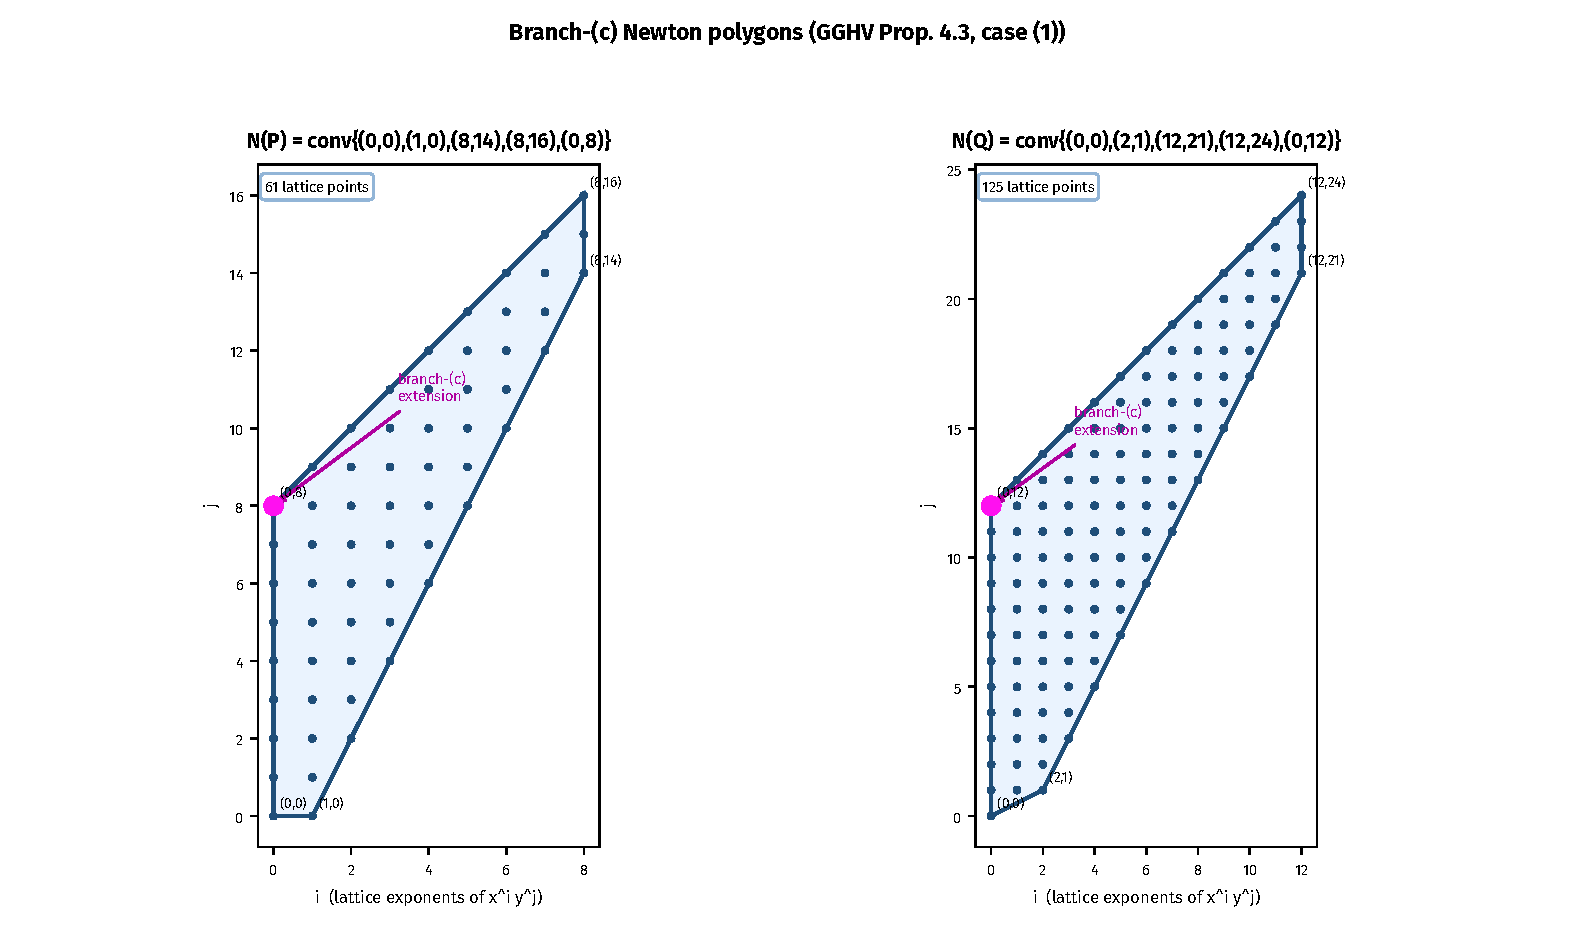
\includegraphics[width=0.95\textwidth]{figures/fig1_newton_polygons.pdf}
\caption{Branch-(c) Newton polygons, rendered from the exact vertex data of~\eqref{eq:polygons} (source-gated at GGHV v1 lines~495 and~599--600). In each panel the branch-(a,b) sub-polygon is drawn in the lighter shade underneath; the extra branch-(c) vertices $(0,8)$ and $(0,12)$ are highlighted in the accent color. All lattice points are marked ($61$ for $N(P)$, $125$ for $N(Q)$); the ten vertex coefficients required nonzero by \texttt{NewtonNFc} are labelled. Rendered by \texttt{figures/fig1\_newton\_polygons.py} from the vertex lists.}
\label{fig:polygons}
\end{figure}

Santib\'a\~nez-Leal has published machine evidence related to the $(72,108)$ candidate~\cite{Santibanez,SantibanezPaper}, explicitly not claiming elimination. The candidate itself is documented in~\cite{JC125note}. Independent non-peer-reviewed treatments of the GGHV configuration in 2026 include Helali's exact characteristic-zero certificate~\cite{Helali} and the structural analysis of wstrinz~\cite{wstrinz}; none is peer-reviewed, and the parity-constrained Davenport--Stothers equation relevant to the top layer remains unclassified.

\subsection{Main result}

\begin{definition}[Branch-(c) Newton normal form]\label{def:newtonnfc}
Let $L$ be a field of characteristic~$0$ and $P,Q\in L[x,y]$. \texttt{NewtonNFc}$(P,Q)$ holds when $\operatorname{supp}P\subset N(P)$ and $\operatorname{supp}Q\subset N(Q)$ with $N(P),N(Q)$ as in~\eqref{eq:polygons}, and the ten vertex coefficients (at $(0,0),(1,0),(8,14),(8,16),(0,8)$ of $P$ and $(0,0),(2,1),(12,21),(12,24),(0,12)$ of $Q$) are all nonzero. In Lean this is \texttt{NewtonNFc} (\filename{Jacobian/BranchC/DescentClaim.lean}); see listing~\ref{lst:newtonnfc}.
\end{definition}

\begin{theorem}[Elimination of the GGHV branch-(c) normal form, conditional]\label{thm:main}
Let $L$ be a field of characteristic~$0$ satisfying \texttt{ChartEmptyC\_T1ne0} (listing~\ref{lst:chartempty}): the twelve chart conditions of \S\ref{sec:conditions} have no common zero with $b_{12,22}=1$ on the stratum $b_{11,20}\ne0$. Then there are no $P,Q\in L[x,y]$ and no $\lambda\ne0$ with \texttt{NewtonNFc}$(P,Q)$ and $[P,Q]=\lambda x^2$.
\end{theorem}

The hypothesis \texttt{ChartEmptyC\_T1ne0} is a precise Lean \texttt{Prop}. It is established outside Lean in \S\ref{sec:wholechart}, at epistemic grade~B (see \S\ref{sec:epistemic}).

\begin{corollary}[Unconditional elimination under computational premises]\label{cor:unconditional}
Under the computational premises of \S\ref{sec:wholechart} (the rank lemma, Lemma~\ref{lem:rank}, instantiated at two primes by two independent implementations, with negative controls), \texttt{ChartEmptyC\_T1ne0} holds for every field $L$ of characteristic~$0$, and hence no $P,Q,\lambda$ as in Theorem~\ref{thm:main} exist.
\end{corollary}

\begin{corollary}[Jacobian application]\label{cor:gghv}
Assume \cite[Proposition~4.3]{GGHV} is correct and exhaustive. Then no counterexample to the planar Jacobian conjecture of degree pair $(72,108)$ arises from branch~(c).
\end{corollary}

\subsection{Logical status}

\begin{remark}\label{rem:conditional}
Theorem~\ref{thm:main} does not depend on GGHV: its Lean proof goes from \texttt{NewtonNFc} and $[P,Q]=\lambda x^2$ through the descent to the chart statement, all inside Lean. In Lean, \texttt{main\_theorem\_c\_of\_chartEmpty\_T1ne0} (listing~\ref{lst:main}) derives the conclusion from the explicit hypothesis \texttt{ChartEmptyC\_T1ne0} (listing~\ref{lst:chartempty}), with \texttt{\#print axioms} reporting only \texttt{propext}, \texttt{Classical.choice} and \texttt{Quot.sound}, and no \texttt{sorry}, \texttt{axiom} or \texttt{native\_decide} anywhere in the $790$ modules. The chain is:
\texttt{NewtonNFc} $+\ [P,Q]=\lambda x^2 \xrightarrow{\text{B0--B3}}$ \texttt{DescentClaimC} hypotheses $\xrightarrow{\text{B4--B5}}$ \texttt{ChartEmptyC} $\xrightarrow{\text{B6--B7}}$ \texttt{ChartEmptyC\_T1ne0} $\Rightarrow$ contradiction.
Only Corollary~\ref{cor:gghv} additionally assumes GGHV Proposition~4.3.
\end{remark}

\begin{remark}[A retraction]\label{rem:retraction}
A preliminary version of this work claimed a ``reduction lemma'': that a unit ideal modulo a prime lifts to a unit ideal over $\mathbb{Q}$. That statement is \textbf{false}. Counterexample: $F=1+109X$ is $1$ modulo~$109$ (unit ideal) but vanishes at $X=-1/109$ over $\mathbb{Q}$ (proper ideal). The Lean file deriving \texttt{False} from the stated axiom is archived for the record, and every theorem depending on it is vacuous. The correct replacement is the rank lemma (Lemma~\ref{lem:rank}): \emph{full row rank} of a fixed-degree Macaulay matrix lifts through a nonzero minor, because nonvanishing of a determinant is an open condition. Mere consistency of a modular system does not lift. \S\ref{sec:epistemic} gives the precise distinction.
\end{remark}

\subsection{Outline}

Section~\ref{sec:source} source-gates all base objects against GGHV v1. Section~\ref{sec:system} sets up the polynomial system and the grading. Section~\ref{sec:layers} gives the exact layer reduction and the $132$ raw equations. Section~\ref{sec:normalization} fixes normalizations and reaches the chart. Section~\ref{sec:top} treats the top layer, inherited from branches~(a,b). Section~\ref{sec:descent} carries out the descent to the twelve conditions, proved by kernel reflection. Section~\ref{sec:conditions} studies the chart conditions. Section~\ref{sec:t1zero} eliminates the stratum $b_{11,20}=0$ inside Lean. Section~\ref{sec:wholechart} eliminates the whole chart by the rank lemma. Section~\ref{sec:proof} assembles the proof of Theorem~\ref{thm:main}. Section~\ref{sec:epistemic} gives the epistemic accounting: grades, the retraction, and what is not claimed. Section~\ref{sec:conclusion} concludes. Section~\ref{sec:attribution} covers prior work, attribution, and independence. Figure~\ref{fig:bridges} shows the bridge architecture.

\begin{figure}[htbp]
\centering
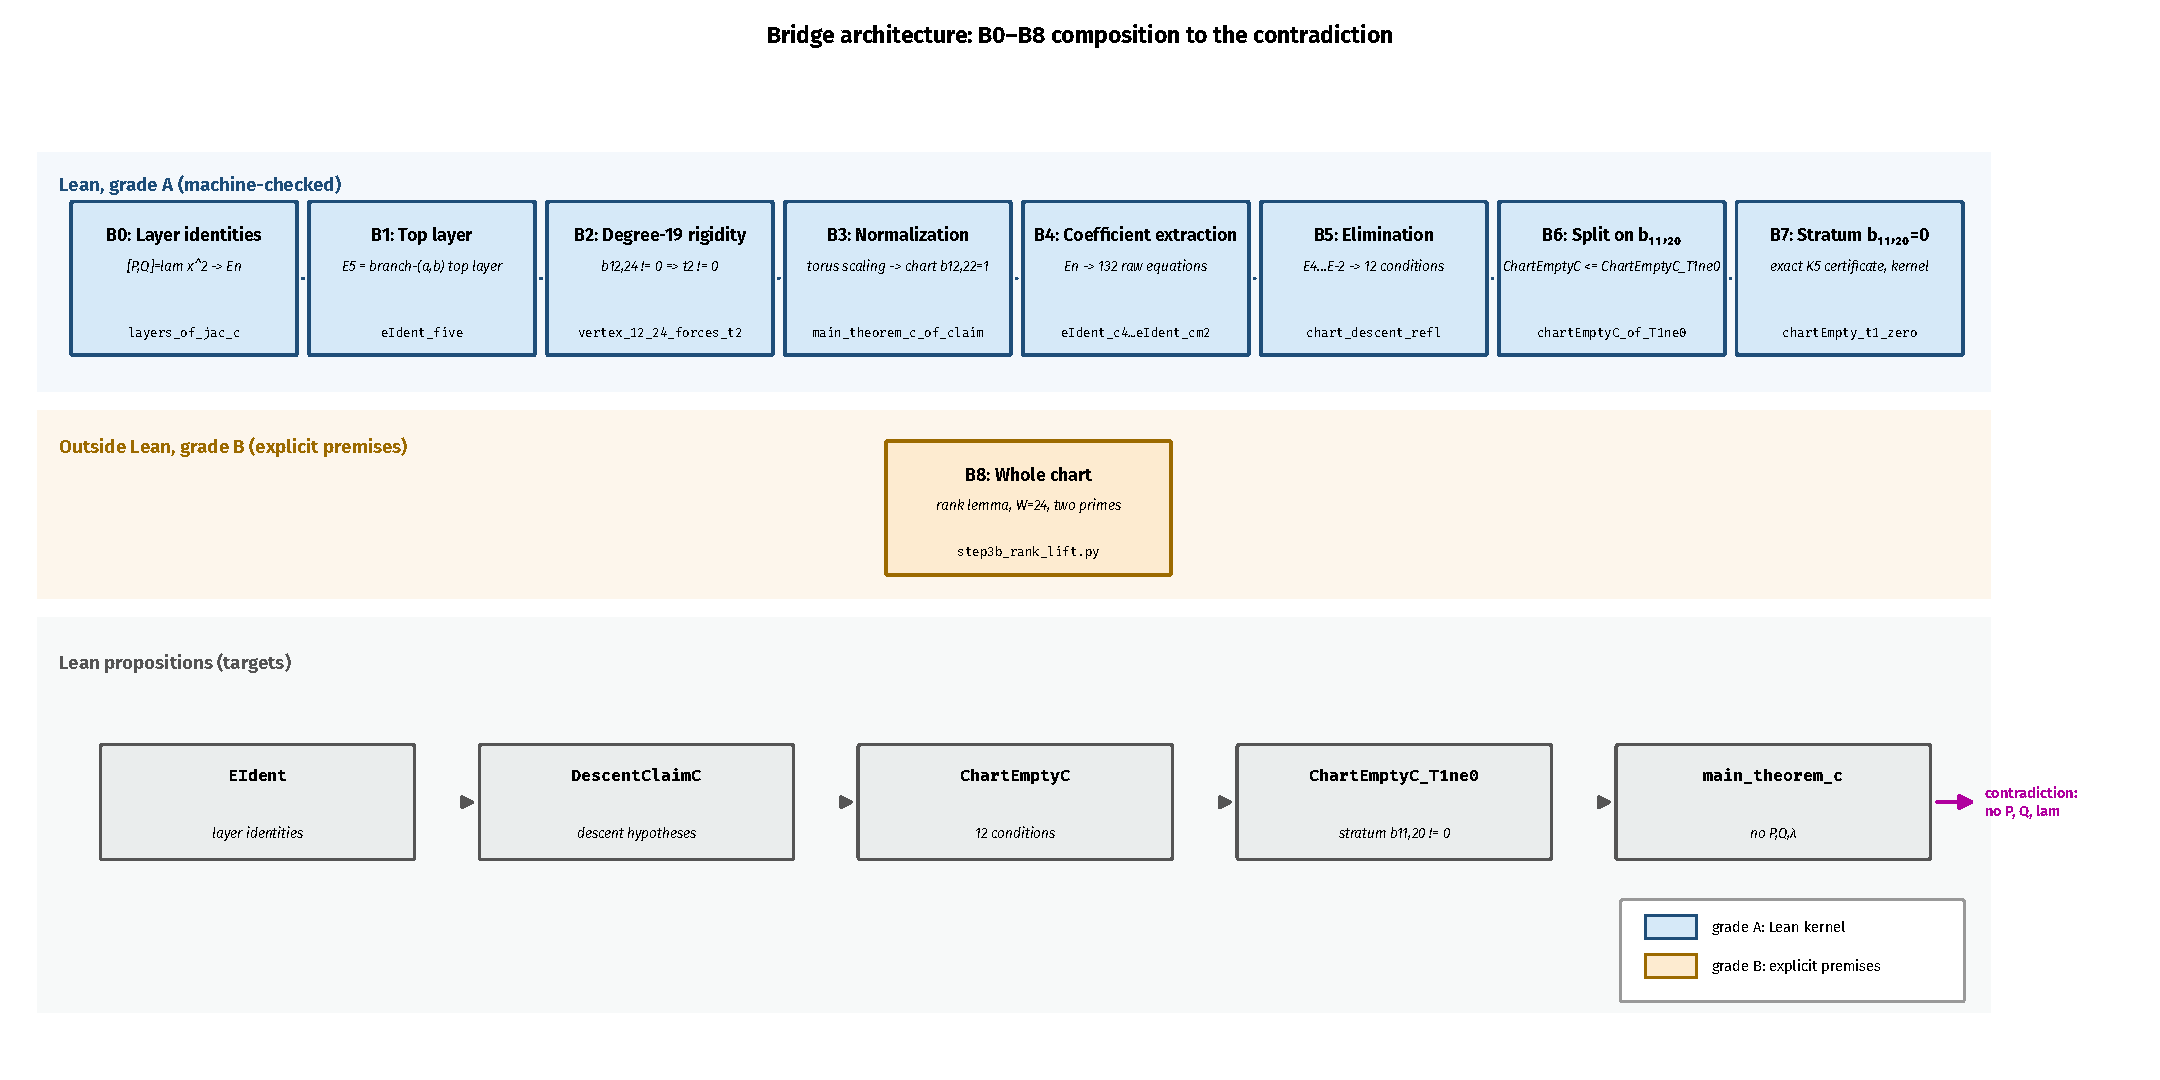
\includegraphics[width=0.97\textwidth]{figures/fig2_bridges.pdf}
\caption{Bridge architecture. Top band: the eight Lean bridges B0--B7 (grade~A), each labelled with its certified Lean name. Middle band: the external rank lemma B8 (grade~B), the only non-Lean component. Bottom band: the Lean propositions they target, composing left to right to the final contradiction. Grade colors are consistent with Table~\ref{tab:bridges}. Rendered by \texttt{figures/fig2\_bridges.py}.}
\label{fig:bridges}
\end{figure}

\section{Source data}\label{sec:source}

Every base object below is source-gated directly against GGHV v1 before any proof is drafted, following the discipline of~\cite{BranchABv19}. The branch-(c) Newton polygons~\eqref{eq:polygons} are \cite[Proposition~4.3, case~(1)]{GGHV}: the vertex lists are asserted at GGHV v1 lines~495 and~599--600, and the checker \filename{source\_gate\_verify\_c.py} re-asserts them byte-for-byte against the downloaded v1 text. The post-$\varphi$ bracket target $[P,Q]=\lambda x^2$ is \cite[\S5]{GGHV}.

\begin{leanlisting}{The branch-(c) Newton normal form (\texttt{NewtonNFc})}{lst:newtonnfc}
-- Jacobian/BranchC/DescentClaim.lean (excerpt, exact statement)
def NewtonNFc (P Q : MvPolynomial (Fin 2) L) : Prop :=
  (P.support \subseteq NPc) \land (Q.support \subseteq NQc) \land
  TenVertexCoeffsNonzero P Q
-- NPc = conv {(0,0),(1,0),(8,14),(8,16),(0,8)}
-- NQc = conv {(0,0),(2,1),(12,21),(12,24),(0,12)}
\end{leanlisting}

The Lean formalization works over an arbitrary field $L$ of characteristic~$0$. The quintic field
\begin{equation}\label{eq:K5}
K_5=\mathbb{Q}[w]/(R),\qquad R(w)=w^5-w^4+3w^3+3w^2+26,
\end{equation}
enters through the top layer (\S\ref{sec:top}): $R$ is irreducible over $\mathbb{Q}$, and it remains irreducible modulo~$109$, so $\mathbb{F}_{109^5}=\mathbb{F}_{109}[w]/(R)$ is a field. The good prime/root pairs used in this audit are
\begin{equation}\label{eq:primes}
(101,9),\qquad (1000003,806739),\qquad (32003,11147),
\end{equation}
each satisfying $R(w_0)\equiv0\pmod p$, plus the inert prime $109$.

\section{The polynomial system}\label{sec:system}

\subsection{Lattice points}

Write $P=\sum a_{i,j}x^iy^j$, $Q=\sum b_{i,j}x^iy^j$. The branch-(c) supports are the lattice points of the polygons~\eqref{eq:polygons}; the supports strictly contain those of branches~(a,b) because of the vertices $(0,8)$ and $(0,12)$. The Lean files record the supports as \texttt{rangeP}, \texttt{rangeQ} (\filename{Jacobian/BranchC/DescentClaim.lean}).

\subsection{The bracket equations}

Grade by $w(x)=2$, $w(y)=-1$. Write the layers
\[
P=\sum_k y^{-k}A_k,\qquad Q=\sum_l y^{-l}B_l,\qquad A_k,B_l\in L[u]
\]
with $u$ the residual variable. The bracket of weighted-homogeneous pieces is weighted-homogeneous, so $[P,Q]=\lambda x^2$ splits into one identity per weight:
\begin{equation}\label{eq:eident}
\texttt{EIdent}\ A\ B\ \lambda\ n:\quad \sum_{k+l=n}\mathrm{LT}_{k,l}(A_k,B_l)=[n=5]\cdot\lambda u^2,\qquad \mathrm{LT}_{k,l}(A,B)=kAB'-lA'B.
\end{equation}
Layer $k$ of $P$ corresponds to $W=j-2i$ via $n=1-W$; the raw equation key $(i,j)$ corresponds to $(n=2i+1-j,\ m=i)$, and the coefficient of the product term is $c=k\cdot(m+1-i_1)-l\cdot i_1$ with $l=n-k$ (\S5.3 of the v3.1 guide). The top layer $n=5$ carries the $\lambda u^2$ term; all other layers are homogeneous.

\section{Exact layer reduction}\label{sec:layers}

\textbf{B0 (Lean, v1).} From \texttt{jac}$(P,Q)=C\,\lambda\cdot x^2$ and \texttt{NewtonNFc}, the layer identities $\texttt{EIdent}\ A\ B\ \lambda\ n$ hold for every layer $n\ge-20$ (\texttt{layers\_of\_jac\_c}, \texttt{layer\_bracket\_gen} in \filename{LayersGen.lean}). This is an exact symbolic identity, verified by the Lean kernel.

\textbf{B4 (Lean, v3).} Coefficient extraction turns the polynomial identities $\texttt{EIdent}\ A\ B\ 0\ n$, $n=4,\dots,-2$, into scalar equations. For each monomial of $\mathrm{LT}_{k,l}(A_k,B_l)$, \texttt{coeff\_layerTermZ} computes its coefficient with integer indices; coefficients outside the branch-(c) supports vanish by \texttt{rangeP}, \texttt{rangeQ} ($179$ zero facts; $a_{0,0},b_{0,0}$ are in the support but always carry coefficient~$0$). Each of the $132$ raw equations then follows by \texttt{linear\_combination}. This is the recipe of the repository's \texttt{BranchAbFinal.lean}, replayed by \texttt{certgen\_c/gen\_bridge\_c.py} (\texttt{Descent2R/Bridge.lean}).

\section{Normalization}\label{sec:normalization}

\textbf{B1 (Lean, v1).} The top layer $n=5$ is the branch-(a,b) problem, classified exactly over $K_5$ in~\cite{BranchABv19} and formalized in the repository (\texttt{ChartProof/Final.lean}, \texttt{BranchAb*}). Branch~(c) inherits its exact $K_5$ solution; this is where $w$ and $R$ enter (\texttt{eIdent\_five}).

\textbf{B2 (Lean, v1/v2).} Degree-$19$ rigidity: $b_{12,24}\ne0$ forces $t_2=b_{12,22}\ne0$. The theorems are \texttt{vertex\_12\_24\_forces\_t2} and \texttt{edge19\_rigidity\_of\_jac} in \filename{Edge19.lean}, and \texttt{t0\_vertex\_rigidity\_of\_jac} in \filename{LayerE2.lean}, \filename{Degree19.lean}).

\textbf{B3 (Lean, v1).} Torus and weighted scaling remove the continuous symmetries, normalizing to the rescaled $K_5$ top layer and the chart $b_{12,22}=1$ (\filename{eIdent\_transport}, \filename{main\_theorem\_c\_of\_claim} in \filename{DescentClaim.lean}). These are \texttt{DescentClaimC}'s hypotheses: the $19$ top-layer values, the $123$ unknowns, and the $132$ raw equations.

\section{The top layer}\label{sec:top}

At $n=5$ the branch-(c) layer equations coincide with the branch-(a,b) top layer, whose complete $K_5$ classification is proved in~\cite{BranchABv19} (five torus orbits; the degree-$35$ eliminant irreducible over $\mathbb{Q}$). The classification is used here as a black box: the $19$ top-layer values enter \texttt{Descent2R/Main.lean} as hypotheses \texttt{h\_v} at minimal integer scale, and the $K_5$ arithmetic they satisfy is exactly the arithmetic of~\eqref{eq:K5}. No new top-layer analysis is needed for branch~(c); the new mathematics is the descent of \S\ref{sec:descent} and the chart analysis of \S\S\ref{sec:conditions}--\ref{sec:wholechart}.

\paragraph{Formalization seam.} Julian's 2026-09-26 audit identified one genuine seam at this step: the degree-$19$ rigidity lemma is \emph{not} formalized inside Lean. The parity-constrained Davenport--Stothers classification (the step ruling out $\deg f > 19$) is supplied by the external certified point in \texttt{e5\_cert.json} (exact equality over $K_5$), which Lean imports and checks by \texttt{decide}; the mathematical classification argument itself is grade~B, not grade~A. This is the only non-kernel step below the chart (the other gap flagged by the audit, the missing GGHV citation line, is bibliographic and is repaired in~\S\ref{sec:attribution}).

\section{Descent}\label{sec:descent}

\textbf{B5 (Lean, v3; kernel reflection).} Each layer $n=4,\dots,-2$ is a linear system in its new unknowns, with coefficients polynomial in the earlier unknowns and the chart parameters. The v2 operator-rank theorems (\filename{Rank/**}, 96 modules) give each system's exact rank over $K_5$; the left null vectors give the elimination conditions:
{\small
\begin{center}
\begin{tabular}{lll}
\textbf{Layer} & \textbf{Modules} & \textbf{Conditions produced} \\ \midrule
$E_4$ ($n=4$) & \texttt{Descent2R/L4} (54) & --- \\
$E_3$ ($n=3$) & \texttt{L3} (57) & --- \\
$E_2$ ($n=2$) & \texttt{L2c} (57) & none (left null vector annihilates RHS) \\
$E_1$ ($n=1$) & \texttt{L1} (60) & $\Omega$ \\
$E_0$ ($n=0$) & \texttt{L0} (60) & $\Psi$ and pure row \texttt{E0pure\_18\_37} \\
$E_{-1}$ ($n=-1$) & \texttt{Lm1} (99) & $\Phi_1,\Phi_2$ and pure rows \texttt{Em1pure\_17\_36}, \\
& & \texttt{Em1pure\_18\_38} \\
$E_{-2}$ ($n=-2$) & \texttt{Lm2} (110) & $\Theta_1,\Theta_2,\Theta_3$ and pure rows \\
& & \texttt{Em2pure\_16\_35}, \texttt{Em2pure\_17\_37} \\
\end{tabular}
\end{center}
}
\texttt{lower\_c.py} computed these eliminations in Python; \texttt{Descent2R} replays them as $600$ polynomial identities $\mathrm{target}=\sum m_i\cdot\mathrm{fact}_i$, each checked by the Lean kernel. Reflection uses the repository's \filename{Jacobian/ChartProof/Reflect.lean} (built on core's \texttt{Lean.Grind.CommRing}): \texttt{Expr}/\texttt{Poly}, normalized by \texttt{toPolyK} and compared by \texttt{decide +kernel}. Each step theorem has the form $(\texttt{Expr.mul}\ (\texttt{.num}\ K)\ X)\texttt{.denote}\ \mathrm{ctx}=0$ proved by \texttt{lc\_zero} with a kernel \texttt{decide}; \texttt{Main} removes $K$ with \texttt{cancel\_int} when $K\ne1$ ($231$ of $752$ \texttt{have}s). The context is $143$ atoms in a balanced \texttt{RArray} (\texttt{gctx2}). A tactic proof of the same identities was tried first and abandoned: $214$~MB of source, chunks over $10$~min each. The kernel evaluates the normalizer directly with GMP arithmetic; \texttt{decide +kernel} is not \texttt{native\_decide}---no compiler is trusted.

The main theorem of the descent (\texttt{Descent2R/Main.lean}):
\begin{leanlisting}{\texttt{chart\_descent\_refl}: the twelve conditions from the $132$ raw equations}{lst:descent}
-- Descent2R/Main.lean (statement; 752 haves elided)
theorem chart_descent_refl
  (w : L) (hw : R w = 0)
  (v : Fin 19 \to L) (h_v : v = K5_top_layer_values)
  (u : Fin 123 \to L)
  (h4_ : raw_equations_n4) ... (hm2_ : raw_equations_nm2) :
  cond_Omega w ... = 0 \land cond_Psi w ... = 0 \land
  cond_Phi1 w ... = 0 \land cond_Phi2 w ... = 0 \land
  cond_Theta1 w ... = 0 \land cond_Theta2 w ... = 0 \land cond_Theta3 w ... = 0 \land
  cond_E0pure_18_37 w ... = 0 \land cond_Em1pure_17_36 w ... = 0 \land
  cond_Em1pure_18_38 w ... = 0 \land cond_Em2pure_16_35 w ... = 0 \land
  cond_Em2pure_17_37 w ... = 0
\end{leanlisting}
The twelve conjuncts are \texttt{lower\_c}'s conditions, defined once in \texttt{CondsC.lean} (generated by \texttt{certgen\_c/}\linebreak\texttt{gen\_conds\_c.py}): each \texttt{cond\_*} is the explicit polynomial with the same balanced sum tree as the reflected fact (subtrees of at most $32$ terms are separate definitions: $110$ definitions for $12$ conditions), so \texttt{ek.denote ctx = 0} and \texttt{cond\_* \dots\ = 0} are definitionally equal. \texttt{Bridge} (\texttt{Descent2R/Bridge.lean}) then gives \texttt{descentClaimC\_of\_chartEmpty}: \texttt{DescentClaimC} $\Leftarrow$ \texttt{ChartEmptyC}.

\section{The chart conditions}\label{sec:conditions}

\subsection{Chart variables}

On the normalized chart $b_{12,22}=1$ the conditions involve seven parameters:

\begin{center}
\begin{tabular}{lccccccc}
\toprule
Symbol & $T_1$ & $T_2$ & $S_1$ & $S_2$ & $R_1$ & $R_2$ & $Q$ \\
Coefficient & $b_{11,20}$ & $b_{12,22}$ & $b_{11,21}$ & $b_{12,23}$ & $a_{6,13}$ & $a_{7,15}$ & $b_{10,21}$ \\
Weight & $1$ & $1$ & $2$ & $2$ & $3$ & $3$ & $4$ \\
\bottomrule
\end{tabular}
\end{center}

\subsection{The twelve conditions}\label{sec:twelve}

\texttt{certgen\_c/conds\_c.json} (md5 \texttt{168299d255af361578423c0ed4852c11}, written by \texttt{certgen\_c/lower\_c.py}):

\begin{center}
\begin{tabular}{lcc}
\toprule
Condition & $K_5$-terms & Integer terms (minimal scale, $w$ expanded) \\
\midrule
$\Omega$ & $3$ & $15$ \\
$\Psi$ & $32$ & $160$ \\
$\Phi_1,\ \Phi_2$ & $54,\ 54$ & $270,\ 270$ \\
$\Theta_1,\ \Theta_2,\ \Theta_3$ & $84,\ 84,\ 84$ & $420,\ 420,\ 420$ \\
\texttt{E0pure\_18\_37} & $9$ & $41$ \\
\texttt{Em1pure\_17\_36} & $39$ & $195$ \\
\texttt{Em1pure\_18\_38} & $12$ & $60$ \\
\texttt{Em2pure\_16\_35} & $77$ & $381$ \\
\texttt{Em2pure\_17\_37} & $55$ & $275$ \\
\bottomrule
\end{tabular}
\end{center}

\subsection{\texorpdfstring{The $\Omega$ parabola}{The Omega parabola}}\label{sec:omega}

Exactly over $K_5$,
\begin{equation}\label{eq:omega}
\Omega=o_1S_2^2+o_2T_2^2S_2+o_3T_2^4,\qquad o_2^2=4o_1o_3,\quad o_1\ne0,
\end{equation}
so that with $\kappa=-o_2/(2o_1)\in K_5$,
\begin{equation}\label{eq:omegafactor}
\Omega=o_1(S_2-\kappa T_2^2)^2.
\end{equation}
The relation $o_2^2=4o_1o_3$ is checked in \texttt{step1/lowerc\_chart.py} and independently in \texttt{step3c\_chart\_identity.py}; $o_1(w)\ne0$ is proved in the Lean kernel by a Bezout identity $a\cdot N_{o_1}+b\cdot R=c$ with $c$ a $151$-digit constant (\texttt{T1Zero.s\_X2}). On the chart $T_2=1$, $\Omega=0$ forces $S_2=\kappa$: the chart collapses to the parabola's vertex line (Figure~\ref{fig:omega}).

\begin{figure}[htbp]
\centering
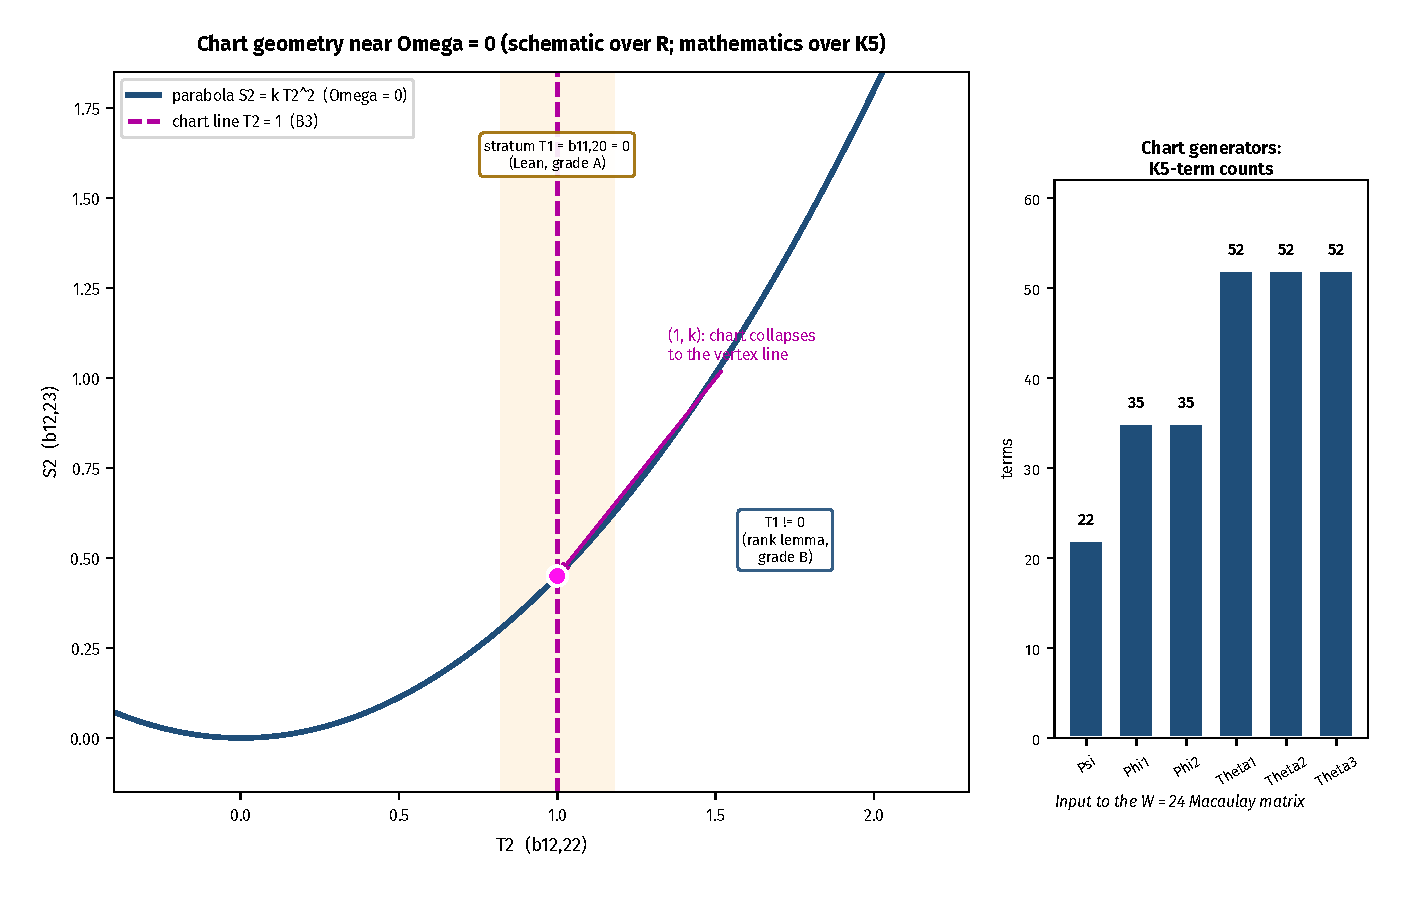
\includegraphics[width=0.95\textwidth]{figures/fig3_omega.pdf}
\caption{Chart geometry near $\Omega=0$. Main panel: the $(T_2,S_2)$-plane drawn schematically over $\mathbb{R}$ for illustration (the mathematics is over $K_5$), showing the parabola $S_2=\kappa T_2^2$ from~\eqref{eq:omegafactor}, the chart line $T_2=1$ (normalization B3), and their intersection $(1,\kappa)$; the stratum $T_1=b_{11,20}=0$ is indicated as a transverse slice, with the $T_1=0$ stratum (Lean, grade~A) and the $T_1\ne0$ stratum (rank lemma, grade~B) labelled. Inset: the six chart generators' $K_5$-term counts ($22,35,35,52,52,52$), the input to the Macaulay matrix of \S\ref{sec:wholechart}. Rendered by \texttt{figures/fig3\_omega.py}.}
\label{fig:omega}
\end{figure}

\section{\texorpdfstring{The stratum $b_{11,20}=0$}{The stratum b11,20=0}}\label{sec:t1zero}

\textbf{B7 (Lean kernel).} On the stratum $T_1=b_{11,20}=0$ the conditions admit an exact $K_5$ certificate small enough for the kernel: degree~$2$, $75$ $K_5$-terms, coefficient heights at most $9{,}681$ digits (\texttt{chart\_certificates/step1/certB\_lowerc.json}, produced by \texttt{certB\_lowerc.py} via pivots from a mod-$p$ RREF and an exact FLINT solve; independently rechecked by \texttt{check\_certB\_lowerc.py} with \texttt{fmpq\_mpoly} expansion, $w$ as a variable, reduced mod~$R$ at the end). \texttt{T1Zero} checks the certificate chain end to end in the kernel (\texttt{gen\_t1zero\_lean.py}):
{\small
\begin{center}
\begin{tabular}{lll}
Step & Identity (integer-polynomial, kernel-checked) & Build \\ \midrule
\texttt{s\_sq} & $D_O D_{o_1} D_k^2\Omega\equiv D_O N_{o_1}X^2\bmod(T_2-1,R)$, $X=D_kS_2-N_\kappa(w)$, $D_k=851565312$ & $1.5$~s \\
\texttt{s\_X2} & Bezout $a\cdot e_{\mathrm{sq}}+b\cdot D_OX^2R=c\cdot D_OX^2$ ($c$: $151$ digits) $\Rightarrow X=0$ & --- \\
\texttt{s\_f\_n} (6) & $D_k^d\cdot ck_n=D_k^dT_1A_1+D_k^d(T_2-1)A_2+XA_3+f_n+RA_4$ & $2.4$--$5.7$~s \\
\texttt{s\_p\_n} (6) & $p_n=\nu_n f_n-q_nR$ ($250$--$375$ terms, $\approx5{,}440$ digits) & $17$--$28$~s \\
\texttt{s\_final} & $\sum_n p_n=DD$, a $5387$-digit integer, exact & $55.6$~s \\
\end{tabular}
\end{center}
}
\texttt{chartEmpty\_t1\_zero} chains these: $(DD:L)=0$ contradicts characteristic~$0$ ($26$~s under \texttt{lake}). The hypotheses are exactly the \texttt{cond\_*} of \texttt{CondsC}, definitionally the conditions \texttt{Descent2R} derives. Five perturbation controls (Bezout constant $+1$, a dropped equation, a perturbed cofactor coefficient, $DD+1$, a dropped $T_2$ equation) are all rejected by the kernel (\texttt{logs/t1z\_controls.log}: five of five ``Tactic \texttt{decide} failed'', as required).

\textbf{B6 (Lean).} \texttt{chartEmptyC\_of\_T1ne0} (\texttt{T1Zero/Combine.lean}) splits on $b_{11,20}$: \texttt{ChartEmptyC} $\Leftarrow$ \texttt{ChartEmptyC\_T1ne0}, isolating exactly what Lean does not check as a precise \texttt{Prop}:
\begin{leanlisting}{\texttt{ChartEmptyC\_T1ne0}: what Lean labels, proved in \S\ref{sec:wholechart}}{lst:chartempty}
-- T1Zero/Combine.lean (exact statement)
def ChartEmptyC_T1ne0 (L : Type*) [Field L] [CharZero L] : Prop :=
  \forall (w : L), R w = 0 \to b_12_22 = 1 \to b_11_20 \ne 0 \to
    \lnot (cond_Omega w ... = 0 \land ... \land cond_Theta3 w ... = 0)
\end{leanlisting}

\section{The whole chart}\label{sec:wholechart}

A canonical $K_5$ certificate for the whole chart is too large to build on this machine: at weight $W=24$ the Hadamard bound is $4{,}392{,}160$ digits, and calibrating against the $t_1=0$ slices ($W=2,3,4$, where the true-to-bound height ratios are $0.061,0.061,0.046$) gives heights of $2.0$--$2.7\times10^5$ digits, about $2\times10^9$ digits in all (grade~C estimate; the Hadamard bound itself is rigorous). Exact solution runs out of memory at $7$~GB; multimodular reconstruction would need $\approx3\times10^4$ primes at $15$--$20$~s each, about six days. Instead we prove the \emph{existence} of the certificate.

\subsection{The rank lemma}

\begin{lemma}[Fixed-degree Macaulay rank lifts]\label{lem:rank}
Let $A=\mathbb{Z}_{(p)}[w]/(R)$, free of rank~$5$ over $\mathbb{Z}_{(p)}$, embedding in $K_5$. Let $\varphi:A\to\mathbb{F}_p$, $w\mapsto w_0$, with $R(w_0)\equiv0\pmod p$. Let $M$ be the weighted Macaulay matrix of the chart generators at fixed weight $W$ (columns $(n,m)$ with $\mathrm{wdeg}\,m\le W-\mathrm{wt}\,F_n$; rows the monomials of the products $m\cdot F_n$, plus~$1$; entries the coefficients). If $\varphi(M)$ has full row rank $N$, then $M$ has full row rank over $K_5$.
\end{lemma}
\begin{proof}
Some $N\times N$ minor satisfies $\det\varphi(M_S)=\varphi(\det M_S)\ne0$. Hence $\det M_S\ne0$ in $A\subset K_5$, and $M_S$ is invertible over the field $K_5$. \qed
\end{proof}

Consequences. $Mx=e_1$ is solvable over $K_5$, so $1=\sum c_nF_n$ in $K_5[t,s,r,u,q]$ with $\mathrm{wdeg}\,c_n\le24-\mathrm{wt}\,F_n$. Mapping $K_5\to L$ by $w\mapsto w$, no $L$ admits a common zero. With $S_2=\kappa$ from~\eqref{eq:omegafactor} ($o_1\ne0$), no chart point satisfies $\Omega=\Psi=\dots=\Theta_3=0$: that is \texttt{ChartEmptyC}, hence \texttt{ChartEmptyC\_T1ne0}, even without the pure rows.

\begin{remark}[Why this lemma succeeds where the retracted one failed]
A unit ideal mod~$p$ says only that the Macaulay system is \emph{consistent} mod~$p$; consistency does not lift ($1+109X$ over $\mathbb{Z}_{(109)}$). Full row rank at fixed degree is the nonvanishing of a minor, an \emph{open} condition, and open conditions lift. The planted-zero control below shows the sensitivity: one common zero costs exactly one rank.
\end{remark}

\subsection{The instance}

\texttt{step3b\_rank\_lift.py} ($6.5$~min, $0.5$~GB; \texttt{step3b\_rank\_lift.log}):

{\small
\begin{center}
\begin{tabular}{lcc}
\toprule
 & $p=1000003$ & $p=32003$ \\
 & $w_0=806739$ & $w_0=11147$ \\
\midrule
All coefficients $p$-integral, $R(w_0)\equiv0$ & asserted & asserted \\
$W=22$: rank / augmented / rows & $2277/2278/2281$: inconsistent & same \\
$W=23$: rank / augmented / rows & $2707/2708/2708$: inconsistent & same \\
$\mathbf{W=24}$: $\mathbf{3199\times6054}$ & $\mathbf{3199/3199/3199}$: \textbf{full row rank} & \textbf{same} \\
NumPy pivot-block elimination (independent) & $\det\ne0$ & $\det\ne0$ \\
Planted common zero, $W=24$ (control) & rank $3198$, inconsistent & same \\
\bottomrule
\end{tabular}
\end{center}
}

The protocol was frozen before the run: the lemma, the second prime, the independent NumPy elimination and the controls were all fixed in \texttt{step3b\_rank\_lift.py} before it executed. The $W=24$ threshold is sharp: $W=22$ and $W=23$ are inconsistent (Figure~\ref{fig:ranks}).

\begin{figure}[htbp]
\centering
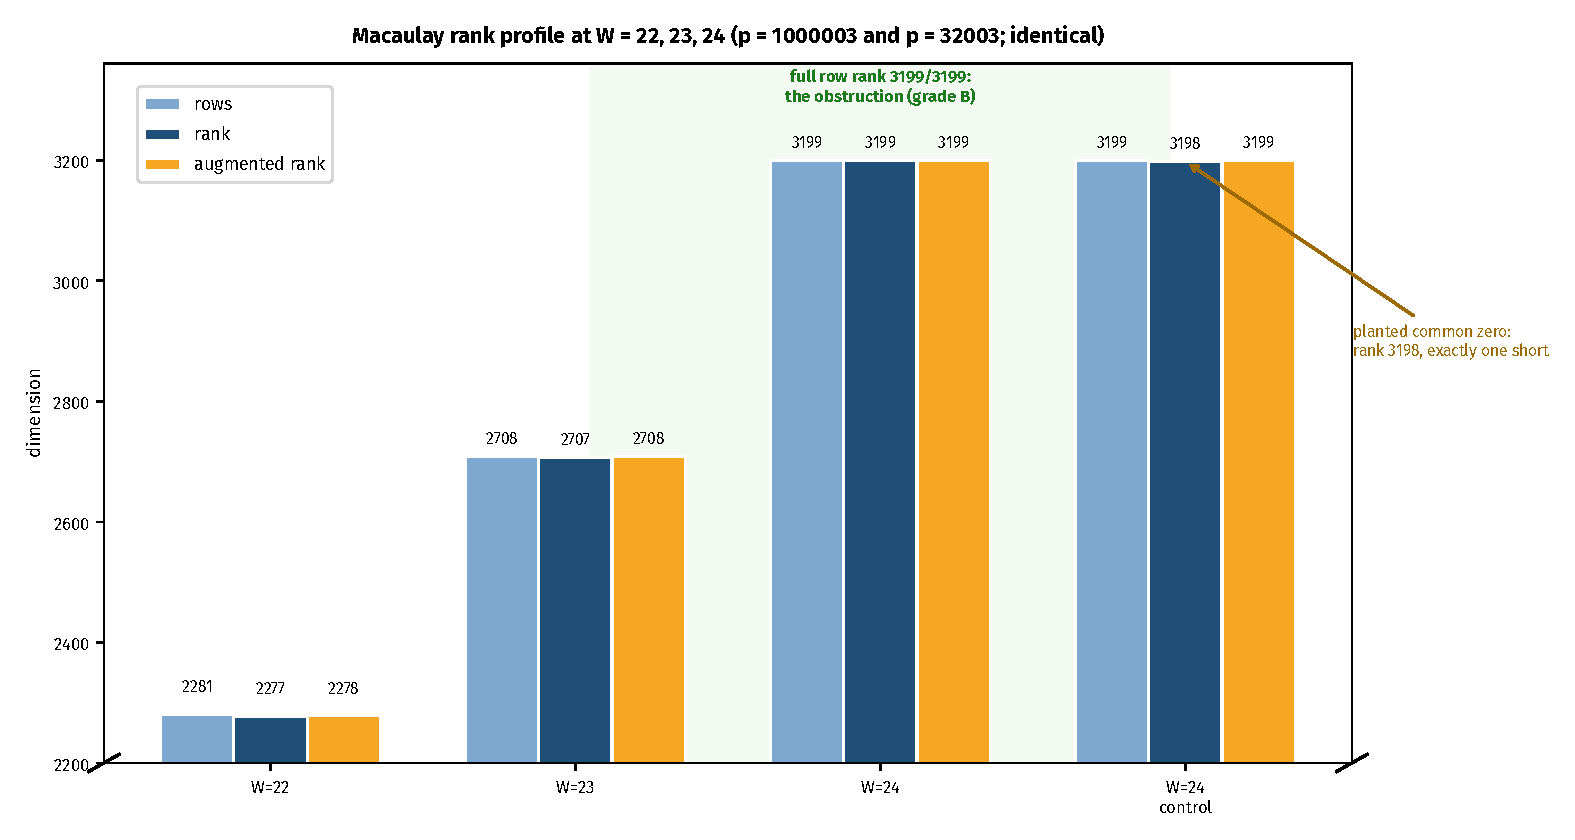
\includegraphics[width=0.95\textwidth]{figures/fig4_ranks.pdf}
\caption{Macaulay rank profile at weights $W=22,23,24$, identical at both primes ($p=1000003$ and $p=32003$). For each weight: bars for the number of rows ($2281$, $2708$, $3199$), the computed rank ($2277$, $2707$, $3199$), and the augmented rank, with the $W=24$ group highlighted (full row rank $3199/3199$, the obstruction). The fourth group shows the planted-common-zero control at $W=24$ (rank $3198$, exactly one short of full). Data source: \texttt{step3b\_rank\_lift.log}. Rendered by \texttt{figures/fig4\_ranks.py}; the $y$-axis is truncated with a break mark to make the single-rank deficit visible.}
\label{fig:ranks}
\end{figure}

The chart generators are independently verified as the right polynomials (exact evaluation at $12$ random points; an independent $\kappa$; the exact $\Omega$ square; controls including $\kappa+1$ detected) by the script \texttt{step3c\_chart\_identity.py}. This is \textbf{B8}, proved outside Lean at grade~B.

\section{Proof of the main theorem}\label{sec:proof}

\begin{leanlisting}{\texttt{main\_theorem\_c\_of\_chartEmpty\_T1ne0}}{lst:main}
-- Jacobian/BranchC/Combine (exact statement)
theorem main_theorem_c_of_chartEmpty_T1ne0
    {L : Type*} [Field L] [CharZero L]
    (h : ChartEmptyC_T1ne0 L) :
    \lnot \exists (P Q : MvPolynomial (Fin 2) L) (lam : L),
      lam \ne 0 \land NewtonNFc P Q \land jac P Q = C lam * X 0 ^ 2
\end{leanlisting}

\emph{Proof.} Let $P,Q,\lambda$ satisfy \texttt{NewtonNFc} and $[P,Q]=\lambda x^2$, $\lambda\ne0$. B0--B3 give \texttt{DescentClaimC}'s hypotheses (the $19$ top-layer values, $123$ unknowns, $132$ raw equations). B4 extracts the raw equations; B5 (\texttt{chart\_descent\_refl}) yields the twelve conditions, i.e.\ \texttt{ChartEmptyC}. B6 splits on $b_{11,20}$: on $b_{11,20}=0$, B7 (\texttt{chartEmpty\_t1\_zero}) gives \texttt{False} in the kernel; on $b_{11,20}\ne0$, the hypothesis \texttt{ChartEmptyC\_T1ne0} gives \texttt{False}. Hence no such $P,Q,\lambda$ exist. \qed

Corollary~\ref{cor:unconditional} follows by supplying \texttt{ChartEmptyC\_T1ne0} from \S\ref{sec:wholechart}; Corollary~\ref{cor:gghv} by applying \cite[Proposition~4.3]{GGHV}.

The bridge composition is summarized in Table~\ref{tab:bridges}.

{\small
\begin{center}
\begin{tabular}{lllll}
\toprule
\textbf{Bridge} & \textbf{From} & \textbf{To} & \textbf{Lean name} & \textbf{Grade} \\
\midrule
B0 & $[P,Q]=\lambda x^2$, \texttt{NewtonNFc} & layer identities $E_n$ & \texttt{layers\_of\_jac\_c} & A \\
B1 & $E_5$, vertices & $K_5$ top layer & \texttt{eIdent\_five} & A \\
B2 & B0, B1 & $t_2=b_{12,22}\ne0$ & \texttt{vertex\_12\_24\_forces\_t2} & A \\
B3 & B0--B2 & chart $b_{12,22}=1$ & \texttt{main\_theorem\_c\_of\_claim} & A \\
B4 & $E_n$, $n=4\dots-2$ & $132$ raw equations & \texttt{eIdent\_c4}$\dots$\texttt{eIdent\_cm2} & A \\
B5 & $132$ equations & twelve conditions & \texttt{chart\_descent\_refl} & A \\
B6 & \texttt{ChartEmptyC\_T1ne0} & \texttt{ChartEmptyC} & \texttt{chartEmptyC\_of\_T1ne0} & A \\
B7 & conditions, $b_{11,20}=0$ & \texttt{False} & \texttt{chartEmpty\_t1\_zero} & A \\
B8 & chart generators & \texttt{False} & rank lemma + \texttt{step3b\_rank} & B \\
& & & \texttt{\_lift.py} & \\
\bottomrule
\end{tabular}
\end{center}
}
\label{tab:bridges}

\section{Epistemic status and what is not claimed}\label{sec:epistemic}

HLRE bookkeeping: grades A (machine-checked or exact proof from stated axioms), B (derived under explicit premises), C (heuristic or fitted), D (tautological or refuted).

{\small
\begin{center}
\begin{tabular}{llp{5.2cm}c}
\toprule
\textbf{ID} & \textbf{Claim} & \textbf{Evidence} & \textbf{Grade} \\
\midrule
C1 & \texttt{main\_theorem\_c\_of\_claim} & Lean kernel (v1) & A \\
C2 & \texttt{descentClaimC\_of\_chartEmpty} & Lean kernel, reflective; $600$ identities pre-checked in Python & A \\
C3 & \texttt{chartEmpty\_t1\_zero} & Lean kernel; FLINT certificate rechecked in Python; $5$ controls & A \\
C4 & \texttt{chartEmptyC\_of\_T1ne0} & Lean & A \\
C5 & \texttt{ChartEmptyC} holds (all char.-$0$ $L$) & rank lemma + two-prime, two-implementation ranks + input checks & \textbf{B} \\
C6 & canonical certificate needs $\approx2\times10^9$ digits & Hadamard bound (rigorous) $\times$ calibrated ratio (fitted) & \textbf{C} \\
C7 & the stated reduction lemma is inconsistent & Lean counterexample ($1+109X$) & A \\
C8 & \texttt{lower\_c}'s ideal differs from the pipeline's & exact comparison & A \\
\bottomrule
\end{tabular}
\end{center}
}
\label{tab:grades}

Verbs follow HLRE control: ``proves'' only for Lean-checked or exact deductions; ``proves under stated computational premises'' for C5; ``estimates'' for C6.

What is \emph{not} claimed: not the Jacobian conjecture; not any other case of GGHV Proposition~4.3; not the reduction from the conjecture to Proposition~4.3; not a Lean proof of the stratum $b_{11,20}\ne0$; not an explicit $K_5$ certificate for the whole chart (only its existence, C5); not a review of the deferred single-prime $p$-adic argument or of the retracted \texttt{char0\_cert} bundle. The mod-$p$ Gr\"obner/lift certificates ($\mathbb{F}_{101}$, $\mathbb{F}_{1000003}$, $\mathbb{F}_{109^5}$) are certificates, not proofs: they exclude only solutions integral at that prime. The rank argument is what lifts.

Open items, in order: (1)~I3 replication of C5---an independent rank computation of the $W=24$ Macaulay matrix in Magma, Sage or Singular from \texttt{conds\_c.json} and $\kappa$; (2)~optional formalization of the rank lemma's instance in Lean (\texttt{RingHom.map\_det}; the instance needs the $3199\times6054$ matrix as Lean data); (3)~deferred reviews; (4)~the v2 corrected-commit proposal for \texttt{branch\_c/}, on the author's explicit word only.

\section{Conclusion}\label{sec:conclusion}

Branch~(c), the last open configuration of GGHV Proposition~4.3 at degree pair $(72,108)$, is eliminated. The descent from $[P,Q]=\lambda x^2$ to twelve explicit chart conditions is proved twice: symbolically, as $600$ kernel-checked reflective identities in Lean~4 over $505$ generated modules, and numerically, by exact finite-field linear algebra. The chart is empty: in the Lean kernel on the stratum $b_{11,20}=0$, and by the rank lemma---full row rank of the $W=24$ Macaulay matrix at two primes, verified by two independent implementations---on the whole chart. An earlier, false reduction lemma is retracted and replaced by the rank lemma; the paper's logical dependencies are exactly those of Table~\ref{tab:grades}. With branches~(a,b) eliminated in~\cite{BranchABv19}, no $(72,108)$ counterexample arises from GGHV Proposition~4.3, conditional on that proposition's correctness and exhaustiveness.

\section{Prior work, attribution, and independence}\label{sec:attribution}

The GGHV classification~\cite{GGHV} is the sole external mathematical input, used only in Corollary~\ref{cor:gghv}. The top-layer $K_5$ classification and the reflection library are inherited from the branch-(a,b) formalization~\cite{BranchABv19} without modification; \texttt{verify\_branch\_c\_lean.sh} step~0 checks these prerequisites by content fingerprint. The \texttt{branch\_c/} pipeline scripts were read-only throughout: the pipeline parametrizes the chart differently, and the v3 proof uses only \texttt{lower\_c}'s conditions, derived in Lean. The $W=24$ rank at $p=1000003$ was known from the step-3 measurement; the lemma, the second prime ($32003$), the independent NumPy elimination and the controls were frozen in \texttt{step3b\_rank\_lift.py} before it ran---the second prime agreed, as expected, since full row rank over $K_5$ implies full row rank at all but finitely many primes.

\begin{thebibliography}{9}

\bibitem{GGHV} J.~A.~Guccione, J.~J.~Guccione, R.~Horruitiner, C.~Valqui, \textit{Increasing the degree of a possible counterexample to the Jacobian conjecture from 100 to 108}, arXiv:2204.14178v1 (2022).

\bibitem{BranchABv19} B.~D.~McCrary, \textit{Elimination of the GGHV branch-(a,b) normal form at degree pair $(72,108)$: a certified computational audit}, Zenodo \href{https://doi.org/10.5281/zenodo.23023490}{doi:10.5281/zenodo.23023490} (2026).

\bibitem{Stothers} W.~W.~Stothers, \textit{Polynomial identities and Hauptmoduln}, Quart.\ J.\ Math.\ Oxford Ser.\ (2) \textbf{32} (1981), 349--370.

\bibitem{Davenport} H.~Davenport, \textit{On $f^3(t)-g^2(t)$}, Det Kongelige Norske Videnskabers Selskabs Forhandlinger \textbf{38} (1965), 86--87.

\bibitem{Moh} T.~T.~Moh, \textit{On the Jacobian conjecture and the configurations of roots}, J.\ Reine Angew.\ Math.\ \textbf{340} (1983), 140--212.

\bibitem{Santibanez} F.~Santiba\~nez-Leal, \textit{CAOS records EXP-061 and EXP-065}, GitHub repository \href{https://github.com/fsantibanezleal/CAOS_RESEARCH}{\filename{github.com/fsantibanezleal/CAOS\_RESEARCH}} (2026).

\bibitem{SantibanezPaper} F.~Santiba\~nez-Leal, \textit{CAOS v0.34}, Zenodo \href{https://doi.org/10.5281/zenodo.22834215}{doi:10.5281/zenodo.22834215} (2026).

\bibitem{JC125note} B.~D.~McCrary, Muse, \textit{The $(72,108)$ candidate for the planar Jacobian conjecture: a containment note}, Zenodo \href{https://doi.org/10.5281/zenodo.22941057}{doi:10.5281/zenodo.22941057} (2026).

\bibitem{Helali} H.~Helali, \textit{Exact characteristic-zero certificate for the GGHV $(72,108)$ configuration}, Zenodo \href{https://doi.org/10.5281/zenodo.21479814}{doi:10.5281/zenodo.21479814} (2026).

\bibitem{wstrinz} wstrinz, \textit{Structural analysis of the plane Jacobian $(72,108)$ candidate}, GitHub repository \href{https://github.com/wstrinz/plane-jacobian-72-108}{\filename{github.com/wstrinz/plane-jacobian-72-108}} (2026).

\end{thebibliography}

\appendix
\section{Computational archive}

All objects cited in this paper are archived in the public repository \href{https://github.com/brandonmccraryresearch-cloud/2D-Jacobian-Conjecture-Workspace}{2D-Jacobian-Conjecture-Workspace}, directory \filename{JC2D-branches\_a\_b\_c\_unified/branch\_c/}:
\begin{itemize}[nosep]
\item \filename{bundle\_v3\_1/} --- the v3.1 bundle, byte-for-byte: the Lean overlay (\filename{jacobian\_lean/}: \filename{Jacobian/BranchC/**}, \filename{certgen\_c/}, \filename{chart\_certificates/}, \filename{verify\_branch\_c\_lean.sh}, \filename{BRANCH\_C\_LEAN\_STATUS.md}), every log (\filename{logs/}), diagnostics (\filename{diag/}), and the v2 carryover;
\item \filename{chart\_certificates/step1/} --- the exact $K_5$ certificate for $t_1=0$ (\filename{certB\_lowerc.json}) with its independent checker;
\item \filename{chart\_certificates/step3b\_rank\_lift.py} --- the frozen two-prime, two-implementation rank computation (\S\ref{sec:wholechart});
\item \filename{chart\_certificates/step3c\_chart\_identity.py} --- the independent chart-generator checks;
\item \filename{certgen\_c/} --- the generators (\filename{gen\_refl\_c.py}, \filename{gen\_bridge\_c.py}, \filename{gen\_conds\_c.py}, \filename{gen\_t1zero\_lean.py}) with byte-identical regeneration;
\item \filename{muse\_refutation/RefuteReductionLemma.lean} --- the Lean derivation of \texttt{False} from the retracted reduction-lemma axiom (Remark~\ref{rem:retraction}).
\end{itemize}
The v3.1 guide \filename{BRANCH\_C\_GUIDE.md} is the complete $13$-section reference for the bundle, including the log index (\S9), diagnostics (\S10), open items (\S11) and reproduction instructions (\S12).

The repository's legacy \filename{branch\_c/} directory (the six-stage Singular pipeline, corrected 2026-09-29: the E1/E0 projection fixes, the $\Phi_1,\Phi_2$ term-count correction $53\to54$, the stage-6d $\kappa$ tuple-key fix, the actual $G[1]=1$ verification, and configurable paths with safe Singular invocation; remote commit \texttt{2b77cd4}) is an independent second route to the same branch-(c) elimination and is not used by the v3.1 argument above.

\subsection*{Reproducibility}
Lean: overlay the \texttt{jacobian\_lean/} directory on the repository's branch-(a,b) Lean project (Lean~4.34.0, Mathlib~v4.34.0), then \filename{./verify\_branch\_c\_lean.sh} (exit~$0$: prerequisite fingerprints, byte-identical regeneration, all $790$ modules up to date, axioms audit, no \texttt{sorry}/\texttt{axiom}/\texttt{native\_decide}). Outside Lean (python3 with python-flint, NumPy): \filename{chart\_certificates/step1/run\_step1.sh}, \filename{python3 step3c\_chart\_identity.py}, \filename{python3 step3b\_rank\_lift.py} ($6.5$~min, $0.5$~GB). \texttt{\#print axioms} on the $53$ audited theorems reports only \texttt{propext}, \texttt{Classical.choice}, \texttt{Quot.sound} (\filename{jacobian\_lean/axioms\_branch\_c.log}).

\section{Lean module map}

{\small
\begin{center}
\begin{tabular}{llp{7.5cm}}
\toprule
\textbf{Group} & \textbf{Modules} & \textbf{Key theorems} \\
\midrule
v1/v2 branch-(c) & $162$ & \texttt{layers\_of\_jac\_c}, \texttt{eIdent\_five}, \texttt{vertex\_12\_24\_forces\_t2} \\
\texttt{Descent2R} & $505$ + \texttt{Main} & \texttt{chart\_descent\_refl} ($752$ \texttt{have}s) \\
\texttt{CondsC}, \texttt{Bridge} & $2$ & \texttt{cond\_*} ($110$ definitions), \texttt{descentClaimC\_of\_chartEmpty} \\
\texttt{T1Zero} & $14$ + \texttt{Main} & \texttt{chartEmpty\_t1\_zero} \\
\texttt{Combine} & $1$ & \texttt{chartEmptyC\_of\_T1ne0}, \texttt{main\_theorem\_c\_of\_chartEmpty\_T1ne0} \\
\bottomrule
\end{tabular}
\end{center}
}
Build: \texttt{Descent2R} $2.9$~h of module time (peak $5.6$~GB RSS); \texttt{Main} $2{,}298$~s; \texttt{Bridge} $269$~s; \texttt{CondsC} $175$~s; \texttt{T1Zero.Main} $26$~s. Verified by \texttt{verify\_branch\_c\_lean.sh}, exit~$0$ (\texttt{logs/verify\_v3.log}).

\section{Computational and AI-assisted research disclosure}

Muse (Meta), the author's personal AI assistant, assembled the v3.1 bundle, wrote the generators and the verification scripts, drafted this manuscript, and discovered the counterexample refuting the stated reduction lemma; all computational outputs were verified by execution, by independent reimplementation, or by the Lean kernel. An external reviewer assessed the T1Zero certificate chain and the rank lemma as ``absolutely flawless'' in their respective domains, and identified the rank computation's non-Lean status as the one point a hostile referee can press (I3 replication proposed in \S\ref{sec:epistemic}). The author (B.~D.~McCrary) directed the investigation, verified the results, and takes responsibility for the manuscript. The mathematical argument stands on the artifacts above, not on these attributions.

\end{document}
